\documentclass[sectionformat=aufgabe]{gadsescript}

\setsemester{Summer Semester 2023/2024}%
\setuniversity{University of Konstanz}%
\settitlelh{\today\\\semester\\Gruppe 3, Jonathan Weihing}
\setfaculty{Faculty of Science\\(Mathematics and Statistics)}%
\settitle{Übungsblatt 3}
\setsubtitle{Elias Gestrich}
\usepackage{subfig}

\begin{document}
\maketitle
\section{Einheitsbälle}
\begin{figure}[h]
	\centering
	\subfloat[]{
		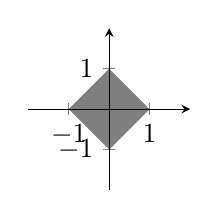
\begin{tikzpicture}
			\begin{axis}[
				xmin= -2, xmax= 2,
				ymin= -2, ymax = 2,
				axis lines = middle,
				xtick = {-1, 0, 1},
				ytick = {-1, 0, 1},
				width = 0.3\textwidth,
				height = 0.3\textwidth,
			]
				% \addplot[domain=-3:3, samples=100]{abs(x) + abs(y) < 1};
				\fill[opacity = 0.5] (1, 0) -- (0, 1) -- (-1, 0) -- (0, -1) -- (1, 0);
			\end{axis}
		\end{tikzpicture}
	}
	\subfloat[]{
		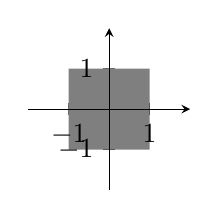
\begin{tikzpicture}
			\begin{axis}[
				xmin= -2, xmax= 2,
				ymin= -2, ymax = 2,
				axis lines = middle,
				xtick = {-1, 0, 1},
				ytick = {-1, 0, 1},
				width = 0.3\textwidth,
				height = 0.3\textwidth,
			]
				% \addplot[domain=-3:3, samples=100]{abs(x) + abs(y) < 1};
				\fill[opacity = 0.5] (1, 1) -- (-1, 1) -- (-1, -1) -- (1, -1) -- (1, 1);
			\end{axis}
		\end{tikzpicture}
	}
	\subfloat[]{
		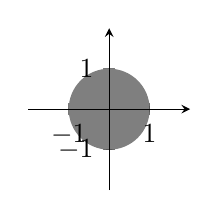
\begin{tikzpicture}
			\begin{axis}[
				xmin= -2, xmax= 2,
				ymin= -2, ymax = 2,
				axis lines = middle,
				xtick = {-1, 0, 1},
				ytick = {-1, 0, 1},
				width = 0.3\textwidth,
				height = 0.3\textwidth,
			]
				% \addplot[domain=-3:3, samples=100]{abs(x) + abs(y) < 1};
				\fill[opacity = 0.5] (0, 0) circle (1);
			\end{axis}
		\end{tikzpicture}
	}\\
	\subfloat[]{
		\begin{tikzpicture}
			\begin{axis}[
				xmin= -2, xmax= 2,
				ymin= -2, ymax = 2,
				axis lines = middle,
				xtick = {-1, 0, 1},
				ytick = {-1, 0, 1},
				width = 0.3\textwidth,
				height = 0.3\textwidth,
			]
				% \addplot[domain=-3:3, samples=100]{abs(x) + abs(y) < 1};
				\fill (0, 0) circle (2pt);
			\end{axis}
		\end{tikzpicture}
	}
	\subfloat[]{
		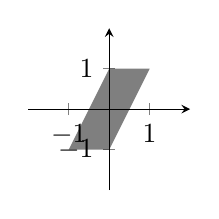
\begin{tikzpicture}
			\begin{axis}[
				xmin= -2, xmax= 2,
				ymin= -2, ymax = 2,
				axis lines = middle,
				xtick = {-1, 0, 1},
				ytick = {-1, 0, 1},
				width = 0.3\textwidth,
				height = 0.3\textwidth,
			]
				% \addplot[domain=-3:3, samples=100]{abs(x) + abs(y) < 1};
			\fill[opacity = 0.5] (-1, -1) -- (0, -1) -- (1, 1) -- (0, 1) -- (-1, -1);
			\end{axis}
		\end{tikzpicture}
	}
\end{figure}

\section{}
\begin{enumerate}[label=(\alph*)]
	\item 
		\begin{description}
			\item[Norm $ \implies  $ konvex:]
				Sei $ x, y \in B $ ($ \left\| x \right\|, \left\| y \right\| \leq 1 $), zu zeigen $ \forall \lambda \in (0, 1) : \left\| \lambda x + ( 1 - \lambda) y \right\| \leq 1 $.
				Sei ein $ \lambda \in (0, 1) $ gegeben, so gilt:
				\begin{align*}
					\left\| \lambda x + ( 1 - \lambda) y \right\| &\leq \left\| \lambda x \right\| + \left\| (1 - \lambda) y \right\| \\
										      &= \lambda \left\| x \right\| + (1 - \lambda) \left\| y \right\|  \\
										      &\leq \lambda + (1 - \lambda) \\
										      &= 1
				 \end{align*}
				 was zu zeigen war.
			 \item[Nicht Norm $ \implies  $ nicht konvex:] 
				 Wenn $ \left\| \cdot  \right\|  $ keine Norm, sondern nur eine Quasinorm ist, zu zeigen $ \exists x, y \in B, \lambda \in [0, 1]: \left\| \lambda x + ( 1 - \lambda) y \right\| > 1 $.\\
				 Da $ \left\| \cdot  \right\|  $ keine Norm, aber eine Quasinorm existiert $ \tilde x, \tilde y \in X : \left\| \tilde x  + \tilde y \right\| > \left\| \tilde x \right\| + \left\| \tilde y \right\|  $, wähle solche $ \tilde x, \tilde y $.
				 \OE{} $ \left\| \tilde x \right\| \geq  \left\| \tilde y \right\|  $.
				 Es folgt:
				 \begin{align*}
					 \left\| \tilde x \right\| + \left\| \tilde y \right\| &< \left\| \tilde x + \tilde y \right\| \\
					 \tag{$ * $}\label{eq:wie labelt man richtig?}
					 1 &< \left\| \frac{ \tilde x }{ \left\| \tilde x \right\| + \left\| \tilde y \right\|  } + \frac{ \tilde y }{ \left\| \tilde x \right\| + \left\| \tilde y \right\|  }  \right\|
				 \end{align*}
				 mit $ 1 \geq  \left\| \frac{ \tilde x }{ \left\| \tilde x \right\| + \left\| \tilde y \right\|  }  \right\| \geq  \left\| \frac{ \tilde y }{ \left\| \tilde x \right\| + \left\| \tilde y \right\|  }  \right\|  $
				 und $ \left\| \frac{ \tilde x }{ \left\| \tilde x \right\| + \left\| \tilde y \right\|  }  \right\| + \left\| \frac{ \tilde y }{ \left\| \tilde x \right\| + \left\| \tilde y \right\|  }  \right\| = \frac{ \left\| \tilde x \right\| + \left\| \tilde y \right\| }{ \left\| \tilde x \right\| + \left\| \tilde y \right\| } = 1 $.\\
				 Wähle $ x \coloneqq  \frac{ \tilde x}{ \left\| \tilde x \right\|  } , y \coloneqq  \frac{ \tilde y }{ \left\| \tilde y \right\|  }  $ und $ \lambda \coloneqq \frac{ \left\| \tilde x \right\| }{ \left\| \tilde x \right\| + \left\| \tilde y \right\| } $, sodass gilt:
				 \begin{align*}
				 	\left\| \lambda x + ( 1 - \lambda) y \right\|
					&= \left\| \frac{ \left\| \tilde x \right\| }{ \left\| \tilde x \right\| + \left\| \tilde y \right\|  } \cdot \frac{ \tilde x }{ \left\| \tilde x \right\|  } + \left( 1 - \frac{ \left\| \tilde x \right\| }{ \left\| \tilde x \right\| + \left\| \tilde y \right\|  }  \right) \cdot \frac{ \tilde y }{ \left\| \tilde y \right\|  }  \right\|  \\
					&= \left\| \frac{ \tilde x }{ \left\| \tilde x \right\| + \left\| \tilde y \right\|  } + \left( \frac{ \left\| \tilde x \right\| + \left\| \tilde y \right\| - \left\| \tilde x \right\| }{ \left\| \tilde x \right\| + \left\| \tilde y \right\|  }  \right) \cdot \frac{ \tilde y }{ \left\| \tilde y \right\|  }  \right\|  \\
					&= \left\| \frac{ \tilde x }{ \left\| \tilde x \right\| + \left\| \tilde y \right\|  } + \left( \frac{ \left\| \tilde y \right\| }{ \left\| \tilde x \right\| + \left\| \tilde y \right\|  }  \right) \cdot \frac{ \tilde y }{ \left\| \tilde y \right\|  }  \right\|  \\
					&= \left\| \frac{ \tilde x }{ \left\| \tilde x \right\| + \left\| \tilde y \right\|  } + \frac{ \tilde y }{ \left\| \tilde x \right\| + \left\| \tilde y \right\|  }  \right\|\\
					&\overset{\eqref{eq:wie labelt man richtig?}}{>} 1\qed
				 \end{align*}
		\end{description}
	\item Für eine Quasinorm ist zu zeigen:
		\begin{enumerate}[label=(\roman*)]
			\item $ \forall x \in \R ^n : \left\| x \right\|_p = 0 \iff x = 0 $:
				\begin{description}
					\item[$ \implies $:] Gegeben $ \left\| x \right\| _p = 0 $, also
						\[
							\sum_{j=1}^{n} \left| x_j \right| ^p = 0 \implies x_j = 0 \quad \forall j = 1, \dotsc, n
						\]
						Was zu zeigen war
					\item[$ \impliedby  $:] trivial.
				\end{description}
			\item $ \forall x \in \R ^n, \lambda \in \R : \left\| \lambda x \right\|_p = \left| \lambda \right| \cdot \left\| x \right\|_p  $:
				\begin{align*}
					\left\| \lambda x \right\| _p &= \left( \sum_{j=1}^{n} \left| \lambda x_j \right| ^p \right) ^{\frac{ 1 }{ p } }  \\
								      &= \left( \sum_{j=1}^{n} \left| \lambda \right|^p \cdot \left| x_j \right| ^p \right) ^{\frac{ 1 }{ p } } \\
								      &= \left( \left| \lambda \right| ^p \sum_{j=1}^{n} \left| x_j \right| ^p \right) ^{\frac{ 1 }{ p } }  \\
								      &= \left( \left| \lambda \right| ^p \right) ^{\frac{ 1 }{ p } } \left( \sum_{j=1}^{n} \left| x_j \right| ^p \right) ^{\frac{ 1 }{ p } }  \\
								      &= \left| \lambda \right| \cdot \left\| x \right\| _p \\
				\end{align*}
			\item $ \exists c \in \R : \forall x, y \in R^n : \left\| x + y \right\|_p \leq c \left( \left\| x \right\| _p + \left\| y \right\| _p \right)  $:\\
				Für $ 1 \leq p < \infty $, ist $ \left\| \cdot  \right\| _p $ laut Vorlesung eine Norm, für $ 0 < p < 1 $:\\
				Sei $ 0 < p < 1 $ gegeben, setze $ p^\prime \coloneqq \frac{ 1 }{ p }  $, so dass $ 1 < p^\prime < \infty $. Es gilt also $ (x^{p^\prime } )^{\prime \prime} = p^\prime (p^\prime -1) x^{p^\prime } > 0 $, also $ x^{p^\prime }  $ konvex, daher gilt, für $ a, b > 0 $:\\
				$ ( a + b )^{p^\prime } \geq  a^{p^\prime }  $ und $ ( a + b)^{p^\prime } \geq b^{p^\prime }  $, daraus folgt $ ( a + b )^{p^\prime } \geq \frac{ 1 }{ 2 } \left( a^{p^\prime } + b^{p^\prime } \right) $, also:
				\begin{align*}
					\frac{ a + b }{ ( a^p + b^p )^{p^\prime }  } &\leq  \frac{ a + b }{ \frac{ 1 }{ 2 } \left( a^{pp^\prime } + b^{pp^\prime } \right) } \\
					&= 2 \frac{ a + b }{ a + b } \\
					&= 2
				\end{align*}
				und
				\begin{align*}
					(a + b)^{p^\prime } &= (0.5 (2a) + 0.5(2b))^{p^\prime }  \\
							    &\leq 0.5 (2a)^{p^\prime } + 0.5 (2b)^{p^\prime } \\
							    &\leq 2^{p^\prime -1} \left(a^{p^\prime } + b^{p^\prime } \right)
				\end{align*}
				Wähle $ c \coloneqq 2^{\frac{ 1 }{ p^2 } }  $, sei $ x, y \in \R ^n $ gegeben
				\begin{align*}
					\left\| x - y \right\| _p &= \left( \sum_{j=1}^{n} \left| x_j - y_j \right|^p \right)^{\frac{ 1 }{ p } }   \\
					~ &\leq \left( \sum_{j=1}^{n} \left( \left| x_j \right| + \left| y_j \right| \right)^p \right) ^{\frac{ 1 }{ p } } \\
					~ &\leq \left( \sum_{j=1}^{n} 2(\left| x_j \right| ^p + \left| y_j \right| ^p ) \right) ^{\frac{ 1 }{ p } } \\
					~ &\leq \left( \sum_{j=1}^{n} 2^{p^\prime } \left| x_j \right|^p  \right) ^{\frac{ 1 }{ p } } + \left( \sum_{j=1}^{n} 2^{p^\prime } \left| y_j \right| ^p \right) ^{\frac{ 1 }{ p } } \\
					~ &\leq 2^{\frac{ 1 }{ p^2 } } \left( \left\| x \right\| + \left\| y \right\|  \right) 
				\end{align*}
				
				
				
				
		\end{enumerate}

		Für $ 0 < p < 1 $ ist der Einheitsball $ B $ nicht konvex, da für
		$ x \coloneqq  \left( 1, 0, \dotsc, 0 \right)  $,
		und $ y \coloneqq \left( 0, 1, 0, \dotsc, 0 \right)  $.
		$ \left\| x \right\| _p = 1 = \left\| y \right\|_p \leq 1 $, also $ x, y \in B $, aber für $ \lambda \coloneqq 0.5 \in [0, 1] $ gilt:
		\begin{align*}
			\left\| \lambda x + ( 1 - \lambda) y \right\|_p &= \left\| \frac{ 1 }{ 2 } x + \frac{ 1 }{ 2 } y \right\|_p  \\
			&= \left\| \left( \frac{ 1 }{ 2 } , \frac{ 1 }{ 2 } , 0, \dotsc, 0 \right)  \right\|_p  \\
			&= \left( 2 \left( \frac{ 1 }{ 2 }  \right) ^p \right) ^{\frac{ 1 }{ p } }  \\
			&= 2^{\frac{ 1 }{ p } } \cdot \frac{ 1 }{ 2 }  \\
			&> 2 \cdot \frac{ 1 }{ 2 }  \\
			&> 1
		\end{align*}

		Für $ p = 1 $ gilt für alle $ x, y \in \R ^n $:
		\begin{align*}
			\left\| x - y \right\| _1 &= \left( \sum_{j=1}^{n} \left| x_j - y_j \right|  \right)  \\
			&\leq \sum_{j=1}^{n} \left| x_j \right| + \sum_{j=1}^{n} \left| y_j \right|  \\
			&\leq \left\| x \right\|_1 + \left\| y \right\|_1
		\end{align*}
		
		Und zuletzt für $ p > 1 $ ist $ \left\| \cdot  \right\| _p $ eine Norm, Beweis in dem Skript
		% da für $ a, b \geq 0: q > 0: (a + b)^q \leq a^q + b^q $
		%\begin{align*}
			%\left\| x + y \right\| &= \left( \sum_{j=1}^{n} \left| x_j + y_j \right| ^p \right) ^{\frac{ 1 }{ p } }  \\
					       %&\leq \left( \sum_{j=1}^{n} \left| x_j \right|^p + \left| y_j \right| ^{p}  \right) ^{\frac{ 1 }{ p } } \\
					       %&\leq \left( \sum_{j=1}^{n} \left| x_j \right|^p + \sum_{j=1}^{n} a_j \left| y_j \right| ^{p}  \right) ^{\frac{ 1 }{ p } } \\
					       %&\leq \left( \sum_{j=1}^{n} \left| x_j \right| ^p \right) ^{\frac{ 1 }{ p } } + \left( \sum_{j=1}^{n} \left| y_j \right| ^p \right) ^{\frac{ 1 }{ p } } 
		%\end{align*}
		
	\item An der {\color{gadse-red}Linie} kann man erkennen, dass der Ball der $ p $-Quasinorm mit $ p = \frac{ 1 }{ 2 }  $ nicht konvex ist, also ist die Quasinorm keine Norm, was nach (b) auch so passt c: (zur Aufgabe 1: Meine Skizzen sind nicht so grob schlecht, dass sie nicht konvex sind, also sind die gezeichneten Skizzen Metriken)
		\begin{figure}[h]
			\centering
			\begin{tikzpicture}
				\begin{axis}[
					xmin= -2, xmax= 2,
					ymin= -2, ymax = 2,
					axis lines = middle,
					width = 8cm,
					height = 8cm,
				]
					% \addplot[domain=-2:2, samples=100]{};
				\fill[domain=-1:1, samples= 101, opacity = 0.5] plot({\x}, {(1 - sqrt(abs(\x)))^2}) -- cycle;
				\fill[domain=-1:1, samples= 101, opacity = 0.5] plot({\x}, {-(1 - sqrt(abs(\x)))^2}) -- cycle;
				\draw[color = gadse-red] (1, 0) -- (0, 1);
				\end{axis}
			\end{tikzpicture}
		\end{figure}
\end{enumerate}

\section{Banachscher Fixpunktsatz}
\begin{enumerate}[label=(\alph*)]
	\item Um zu zeigen, dass $ f(x) = x $ genau eine Lösung in $ [1, \infty] $ besitzt reicht zu zeigen, dass $ f $ von $ [1, \infty) $ auf $ [1, \infty] $ abbildet und $ \exists 0 \leq L < 1 : \forall x, y \in [1, \infty) : d(f(x), f(y)) \leq L d(x, y) $ mit $ d(x, y) \coloneqq \left| x - y \right|  $:
		\begin{description}
			\item[Wertebereich:] Für $ 1 \leq x < 2 : f(x) = \frac{ 1 }{ 2 } \left(x + \frac{ 2 }{ x } \right) \geq  \frac{ 1 }{ 2 } \left( 1 + \frac{ 2 }{ 2 }  \right) = 1 $
				und für $ 2 \leq x : f(x) = \frac{ 1 }{ 2 } \left( x + \frac{ 2 }{ x }  \right) \geq \frac{ 1 }{ 2 } \left( 2 + 0 \right) = 1 $ \qed
			\item[Kontraktion:] Sei $ L \coloneqq \frac{ 1 }{ 2 }  $, sei $ x, y \in [1, \infty) $ beliebig zu zeigen $ \left| f(x) - f(y) \right| \leq L \left| x - y \right|  $:
				\begin{align*}
					\left| f(x) - f(y) \right| &= \left| \frac{ 1 }{ 2 } \left( x + \frac{ 2 }{ x }  \right) + \frac{ 1 }{ 2 } \left( y + \frac{ 2 }{ y }  \right)  \right|  \\
								   &= \frac{ 1 }{ 2 } \left| x - y - \left( \frac{ 2 }{ y } + \frac{ 2 }{ x }  \right)  \right| \\
								   &= \frac{ 1 }{ 2 } \left| \left( x - y \right) - 2 \left( \frac{ x - y }{ xy }  \right)  \right|  \\
								   &= \frac{ 1 }{ 2 } \left| \frac{ (xy) ( x - y ) - 2 (x - y) }{ xy }  \right|  \\
								   &= \left| \frac{ xy - 2 }{ xy }  \right| \cdot \frac{ 1 }{ 2 } \cdot \left| x - y \right|  \\
								   &= \left| 1 - \frac{ 2 }{ xy }  \right| \cdot \frac{ 1 }{ 2 } \cdot \left| x - y \right|  \\
								   &\leq \frac{ 1 }{ 2 } \left| x - y \right| 
				\end{align*}
		\end{description}
	\item Es gilt $ f\left( \sqrt{2}  \right) = \frac{ 1 }{ 2 } \left( \sqrt{2} + \frac{ 2 }{ \sqrt{2}  }  \right) = \frac{ 1 }{ 2 } \left( \sqrt{2} + \frac{ 2 \sqrt{2} }{ 2 }  \right) = \sqrt{2}  $. Zu beweis siehe (c) (für $ \varepsilon > 0 $ wähle $ N $, so dass $ - \frac{ \ln \varepsilon }{ \ln 2  } < N $, der Rest ergibt sich dann)
	\item Beweis durch vollständige Induktion:
		\begin{description}
			\item[I.A.: $ n = 0 $:] $ \left| x_n - \sqrt{2}  \right| = \left| x_0 - \sqrt{2}  \right| = \left| 1 - \sqrt{2}  \right| < \left| -0.5 \right| = \frac{ 1 }{ 2 } = 2^{-1} $ 
			\item[I.S.: $ n \curvearrowright n + 1 $:]
				\begin{description}
					\item[I.V.:] $ \left| x_n - \sqrt{2}  \right| \leq 2^{-n}  $.
				\end{description}
				Zu zeigen $ \left| x_{n+1} - \sqrt{2}  \right| \leq 2^{-(n+1)}  $
				\begin{alignat*}{2}
					&\left| x_{n + 1} - \sqrt{2} \right| &\omit\hfill$ = $\hfill& \left| f(x_n) - f(\sqrt{2} ) \right|  \\
					&&\omit\hfill$\overset{\text{(a), (b)} }{\leq }$\hfill& \frac{ 1 }{ 2 } \left| x_n - \sqrt{2}  \right| \\
					&&\omit\hfill$\overset{\text{I.V.} }{\leq }$\hfill& \frac{ 1 }{ 2 } 2^{-n} \\
					&&\omit\hfill$\leq$\hfill& 2^{-(n+1)} \qed
				\end{alignat*}
		\end{description}
\end{enumerate}

\section{Vollständigkeit}
\begin{enumerate}[label=(\alph*)]
	\item 
		\begin{description}
			\item[$ c_{00}(\N ) \subsetneq \bigcap_{i \leq q \leq \infty} l^q(\N ) $:] Für $ c_{00} (\N ) \subseteq \bigcap_{i \leq q \leq \infty} l^q(\N ) $: Sei $ (x_j) \subset \R : \exists N \in \N : \forall j \geq N : x_j = 0 $, zu zeigen $ \left\| (x_j) \right\| _p < \infty $:
				\begin{align*}
					\left\| (x_j) \right\| _p &= \left( \sum_{j=1}^{n} \left| x_j \right| ^p \right) \frac{ 1 }{ p }  \\
					&= \left( \sum_{j=1}^{N} \left| x_j \right| ^p \right) ^{\frac{ 1 }{ p } }  \\
				\end{align*}
				Da  $ \sum_{j=1}^{N} \left| x_j \right| < \infty $ ist auch $ \left\| x_j \right\| < \infty $, was zu zeigen war, für $ c_{00}(\N ) \neq \bigcap_{i \leq q \leq \infty} l^q(\N ) $:
				\begin{align*}
					\left\| \left( \frac{ 1 }{ 2 }  \right) ^j \right\| _p &= \left( \sum_{j=1}^{\infty} \left| \frac{ 1 }{ 2 }  \right|^{jp}   \right) ^{\frac{ 1 }{ p } }  \\
				       &\leq \bigg( \underbrace{\sum_{j=1}^{\infty} \left( \frac{ 1 }{ 2 }  \right) ^j}_{= \frac{ 1 }{ 1 - 2 } -1 = 1} \bigg) ^{\frac{ 1 }{ p } } \\
					&\leq 1 < \infty
				\end{align*}
			\item[$ \bigcap_{i \leq q \leq \infty} l^q(\N ) \subset l^p(\N ) $:] trivial
			\item[$ l^p(\N ) \subsetneq c_0(\N ) $:] 
				\begin{description}
					\item[$ \subset  $:] Sei $ (x_j) \in l^p(\N ) $, zu zeigen $ x \in c_0(\N ) $.
						Beweis durch Widerspruch, wir nehmen an, $ x \not\in c_0(\N ) $, also $ (x_j) $ keineNullfolge.
						Also $ \exists \varepsilon > 0 : \forall N \in \N : \exists n > N : \left| x_j \right| > \varepsilon $,
						sei $ (x_{a_j} ) $, eine Teilfolge von $ (x_j) $ mit $ a_j < a_{j+1}  $ und $ \forall j \in \N : | x_{a_j} | > \varepsilon $,
						diese existiert, da $ \forall a_j \in \N : n > a_j : \left| x_n \right| > \varepsilon  $,
						also $ \sum_{j=1}^{\infty} \left| x_{a_j} \right| = \infty $,
						also auch $ \sum_{j=1}^{\infty} \left| x_j \right| = \infty \implies \sum_{j=1}^{\infty} \left| x_j \right| ^p = \infty \implies \left( \sum_{j=1}^{\infty} \left| x_j \right| ^p \right) ^{\frac{ 1 }{ p } } = \infty $
					\item[$ \neq  $] Sei $ (x_j) = ( \frac{ 1 }{ j } )^{\frac{ 1 }{ p } }  $, sodass gilt:
						\begin{align*}
							\left\| x_j \right\| _p &= \left( \sum_{j=1}^{\infty} \left| \left( \frac{ 1 }{ j }  \right) ^{\frac{ 1 }{ p } }  \right| ^p \right) ^{\frac{ 1 }{ p } } \\
										&= \left( \sum_{j=1}^{\infty} \frac{ 1 }{ j }  \right) ^{\frac{ 1 }{ p } } \\
										&= \infty^{\frac{ 1 }{ p } }  \\
										&= \infty \\
						\end{align*}
						Also $ (x_j) $ nicht in $ l^p(\N ) $, aber $ \left( \frac{ 1 }{ j }  \right) ^{\frac{ 1 }{ p } }  $ geht gegen Null.
				\end{description}
			\item[$ c_0(\N ) \subsetneq l^\infty(\N ) $:] Alle Nullfolgen sind trivialer weise beschränkt, zu zeigen $ \exists (x_j) \in l^\infty(\N ) : (x_j) \not\in c_0(\N ) $. Wähle die konstante Folge $ (x_j) = 1 \forall j \in \N  $, sodass $ (x_j) $ durch 1 nach unten und oben beschränkt ist, aber $ (x_j) $ konvergiert trivialer weiße nicht gegen 0\qed
		\end{description}
	\item Da ich nicht weiß, wie man Folgen von Folgen aufschreibt, habe ich mit $ ((x_j)_n) $ eine Folge einer Folge gemeint, mit den Folgengliedern $ (x_j)_n $, welche selbst Folgen sind und die Folgenglieder $ x_{j, n}  $ haben.\\
		$ c_{00}(\N )  $ ist nicht in $ d_p $ vollständig, da $ c_{00}(\N ) $ in $ d_p $ nicht abgeschlossen ist, da die Folge $ ((x_j)_n) $ mit
		\[ x_{j,n} \coloneqq  \begin{cases}
				\left( \frac{ 1 }{ 2 }\right)^j , & \quad \text{wenn } j < n\\
				0, & \quad \text{sonst} 
			\end{cases}
		\]
		$ d_p $-Cauchy ist, sei $ \varepsilon > 0 $ gegeben, setze, setze $ N > \frac{ \ln \varepsilon }{ \ln \frac{ 1 }{ 2 } } \cdot p  + 1 $, sodass $ \left( \frac{ 1 }{ 2 }  \right) ^{\frac{N - 1}{ p } }  < \varepsilon $, sodass für alle $ l, k \in \N  $ \OE{} $ l < k $, und gilt:
		\begin{align*}
			d_p((x_j)_l, (x_j)_k) &= \left( \sum_{j=l}^{k} \left| \left( \frac{ 1 }{ 2 }  \right) ^j \right| ^p \right) ^{\frac{ 1 }{ p } }  \\
			&\leq \left( \sum_{j=N}^{\infty} \left( \frac{ 1 }{ 2 }  \right) ^{pj}  \right) ^{\frac{ 1 }{ p } }  \\
			&\leq \left( \frac{ 1 }{ 2^{N - 1} } \sum_{j=1}^{\infty} \left( \frac{ 1 }{ 2 }  \right) ^{pj}  \right) ^{\frac{ 1 }{ p } }  \\
			&\leq \left( \frac{ 1 }{ 2^{N - 1} } 1  \right) ^{\frac{ 1 }{ p } }  \\
			&\leq \frac{ 1 }{ 2^{\frac{N - 1}{ p } } } \\ 
			&\leq \varepsilon 
		\end{align*}
		die Folge ist auch $ d_{\infty}  $-Cauchy, da $ \sup(|x_{j, l}|) = \sup(| x_{j, k}| ) = \frac{ 1 }{ 2 } $, also $ d_\infty((x_j)_l , (x_j)_k ) = 0 $.
		Aber für $ n \to \infty $ geht $ ((x_{j})_n )  $ gegen $ \left( \frac{ 1 }{ 2^j } \right) $ und $ \left| \left( \frac{ 1 }{ 2^j }  \right)  \right| > 0 $ für alle $ j \in \N $, somit $ \lim_{n \to \infty}  (x_j)_n \not\in c_{00}(\N ) $
	\item 
		\begin{description}
			\item[Nicht vollständig bezüglich $ d_\infty $:] Sei $ (x_{j, n}) \coloneqq ((x_j)_n) $ mit
				\[
					x_{j, n}  = \begin{cases}
						1, &\quad \text{für } j < n\\
						0, &\quad \text{sonst} 
					\end{cases}
				\]
				Dann für alle $ l, k \in \N : d_{\infty} ((x_{l, n} ), (x_{j, k})) = d_{\infty} (1, 1) = 0  $
				Also $ d_\infty $-Cauchy, aber da $ (x_j) $ mit $ x_j = 1 $ die Grenzfolge für $ ((x_j)_n) $ ist und:
				\begin{align*}
					\left\| (x_j) \right\| _p &= \left( \sum_{j=1}^{\infty} 1^p \right) ^{\frac{ 1 }{ p } }  \\
					&= \infty^{\frac{ 1 }{ p } }  \\
					&\nless \infty
				\end{align*}
			\item[Vollständigkeit bezüglich $ d_p $:]
				Sei $ ((x_j)_n) $ $ d_p $-Cauchy, zu zeigen $ \lim_{n \to \infty} ((x_j)_n) \in l^p(\N ) $, also $ \lim_{n \to \infty} \left( \sum_{j=1}^{\infty} \left| x_{j, n}  \right| ^p \right) ^{\frac{ 1 }{ p } } < \infty $.\\
				Da $ ((x_j)_n) $ $ d_p $-Cauchy
		\end{description}
		
		
\end{enumerate}


\end{document}
